\documentclass[aspectratio=169,10pt]{beamer}
\usepackage{mathptmx}
\usepackage{booktabs}
\usepackage{graphicx}
\usefonttheme{serif}
\setbeamertemplate{navigation symbols}{}
\setbeamertemplate{footline}{\hfill\tiny\insertframenumber\hspace{6pt}\vspace{4pt}}
\setbeamercolor{frametitle}{fg=black}
\setbeamerfont{frametitle}{size=\normalsize,series=\bfseries}
\setbeamertemplate{itemize items}{\textbullet}
\graphicspath{{../figures/}{slides/}}

% One layout for every RQ slide: question as title, figure box left (fixed size), bullets right.
\newcommand{\rqslide}[5]{%
\begin{frame}{#1\quad #2}
\begin{columns}[T,onlytextwidth]
\begin{column}{0.56\textwidth}
\centering
\includegraphics[width=\linewidth,height=0.74\textheight,keepaspectratio]{#3}\\[-1pt]
{\tiny\textit{#4}}
\end{column}
\begin{column}{0.41\textwidth}
\footnotesize
#5
\end{column}
\end{columns}
\end{frame}}

\title{Research questions from the current analysis}
\subtitle{Multimodal drivers + TerraMind embeddings for daily soil moisture}
\author{Prajwal Khanal}
\date{7 October 2026}

\begin{document}

\begin{frame}
\titlepage
\end{frame}

%---------------- Motivation (slides 1-5 live in slides/motivation_frames.tex)
% Motivation slides 1-4, shared by text/research_questions_slides.tex and text/slides/motivation_slides.tex
\begin{frame}{Motivation\quad Different ways of obtaining soil moisture}
\scriptsize
\centering
\renewcommand{\arraystretch}{1.25}
\begin{tabular}{@{}p{0.14\textwidth} p{0.26\textwidth} p{0.16\textwidth} p{0.34\textwidth}@{}}
\toprule
Source & How SM is obtained & Depth & Main limitation \\
\midrule
\textbf{Microwave}\newline (SMAP, SMOS, ASCAT, S1)
  & invert:\newline $\sigma^0$ or $T_B = f(\mathrm{SM}, \text{roughness}, \text{vegetation})$
  & top $\sim$5\,cm; informs part of the root zone (Feldman et al., 2023)
  & shallow; assumes vegetation and roughness; coarse (9--40\,km) except S1 \\
\addlinespace[7pt]
\textbf{Optical / thermal}\newline (S2, Landsat, MODIS)
  & empirical relations with surface properties: reflectance and indices; LST--vegetation space (e.g. triangle method, TVDI)
  & skin / surface
  & indirect, site-specific calibration; clouds; canopy hides the soil \\
\addlinespace[7pt]
\textbf{Land-surface models}
  & $d\theta/dt = P - ET - Q - D$, with parameters $p$
  & full profile
  & forcing errors, soil and vegetation parameters, process representation (Koster et al., 2009; Seneviratne et al., 2010) \\
\addlinespace[7pt]
\textbf{Reanalysis}\newline (ERA5-Land)
  & LSM driven by reanalysis meteorology
  & full profile
  & model assumptions dominate deep layers with few observational constraints (Li et al., 2021; Miguez-Macho and Fan, 2021) \\
\addlinespace[7pt]
\textbf{In situ} (ISMN)
  & direct probe measurement
  & several depths
  & point scale; sparse, uneven global coverage \\
\addlinespace[7pt]
\textbf{Data-driven}\newline (ML / DL)
  & $\mathrm{SM} = f_\theta(\text{inputs})$, learned from in-situ labels; no ad-hoc process assumptions
  & any depth with labels
  & needs enough, representative sites; generalisation?; hard to interpret? \\
\bottomrule
\end{tabular}
\end{frame}

\begin{frame}{Motivation\quad Multimodal remote sensing}
\begin{columns}[T,onlytextwidth]
\begin{column}{0.56\textwidth}
\centering
\textbf{\footnotesize 1.\ Optical: reflectance spectrum}\\[2pt]
\includegraphics[width=\linewidth,height=0.42\textheight,keepaspectratio]{textbook/sm_signals.pdf}
\scriptsize
\begin{itemize}
\item Dry and wet soil reflect differently: wetting darkens soil in every band, most in the SWIR (B11, B12)
\item Green and water-stressed vegetation reflect differently: stress lowers NIR and raises SWIR
\end{itemize}
\end{column}
\begin{column}{0.41\textwidth}
\centering
\textbf{\footnotesize 2.\ SAR: scattering mechanisms}\\[2pt]
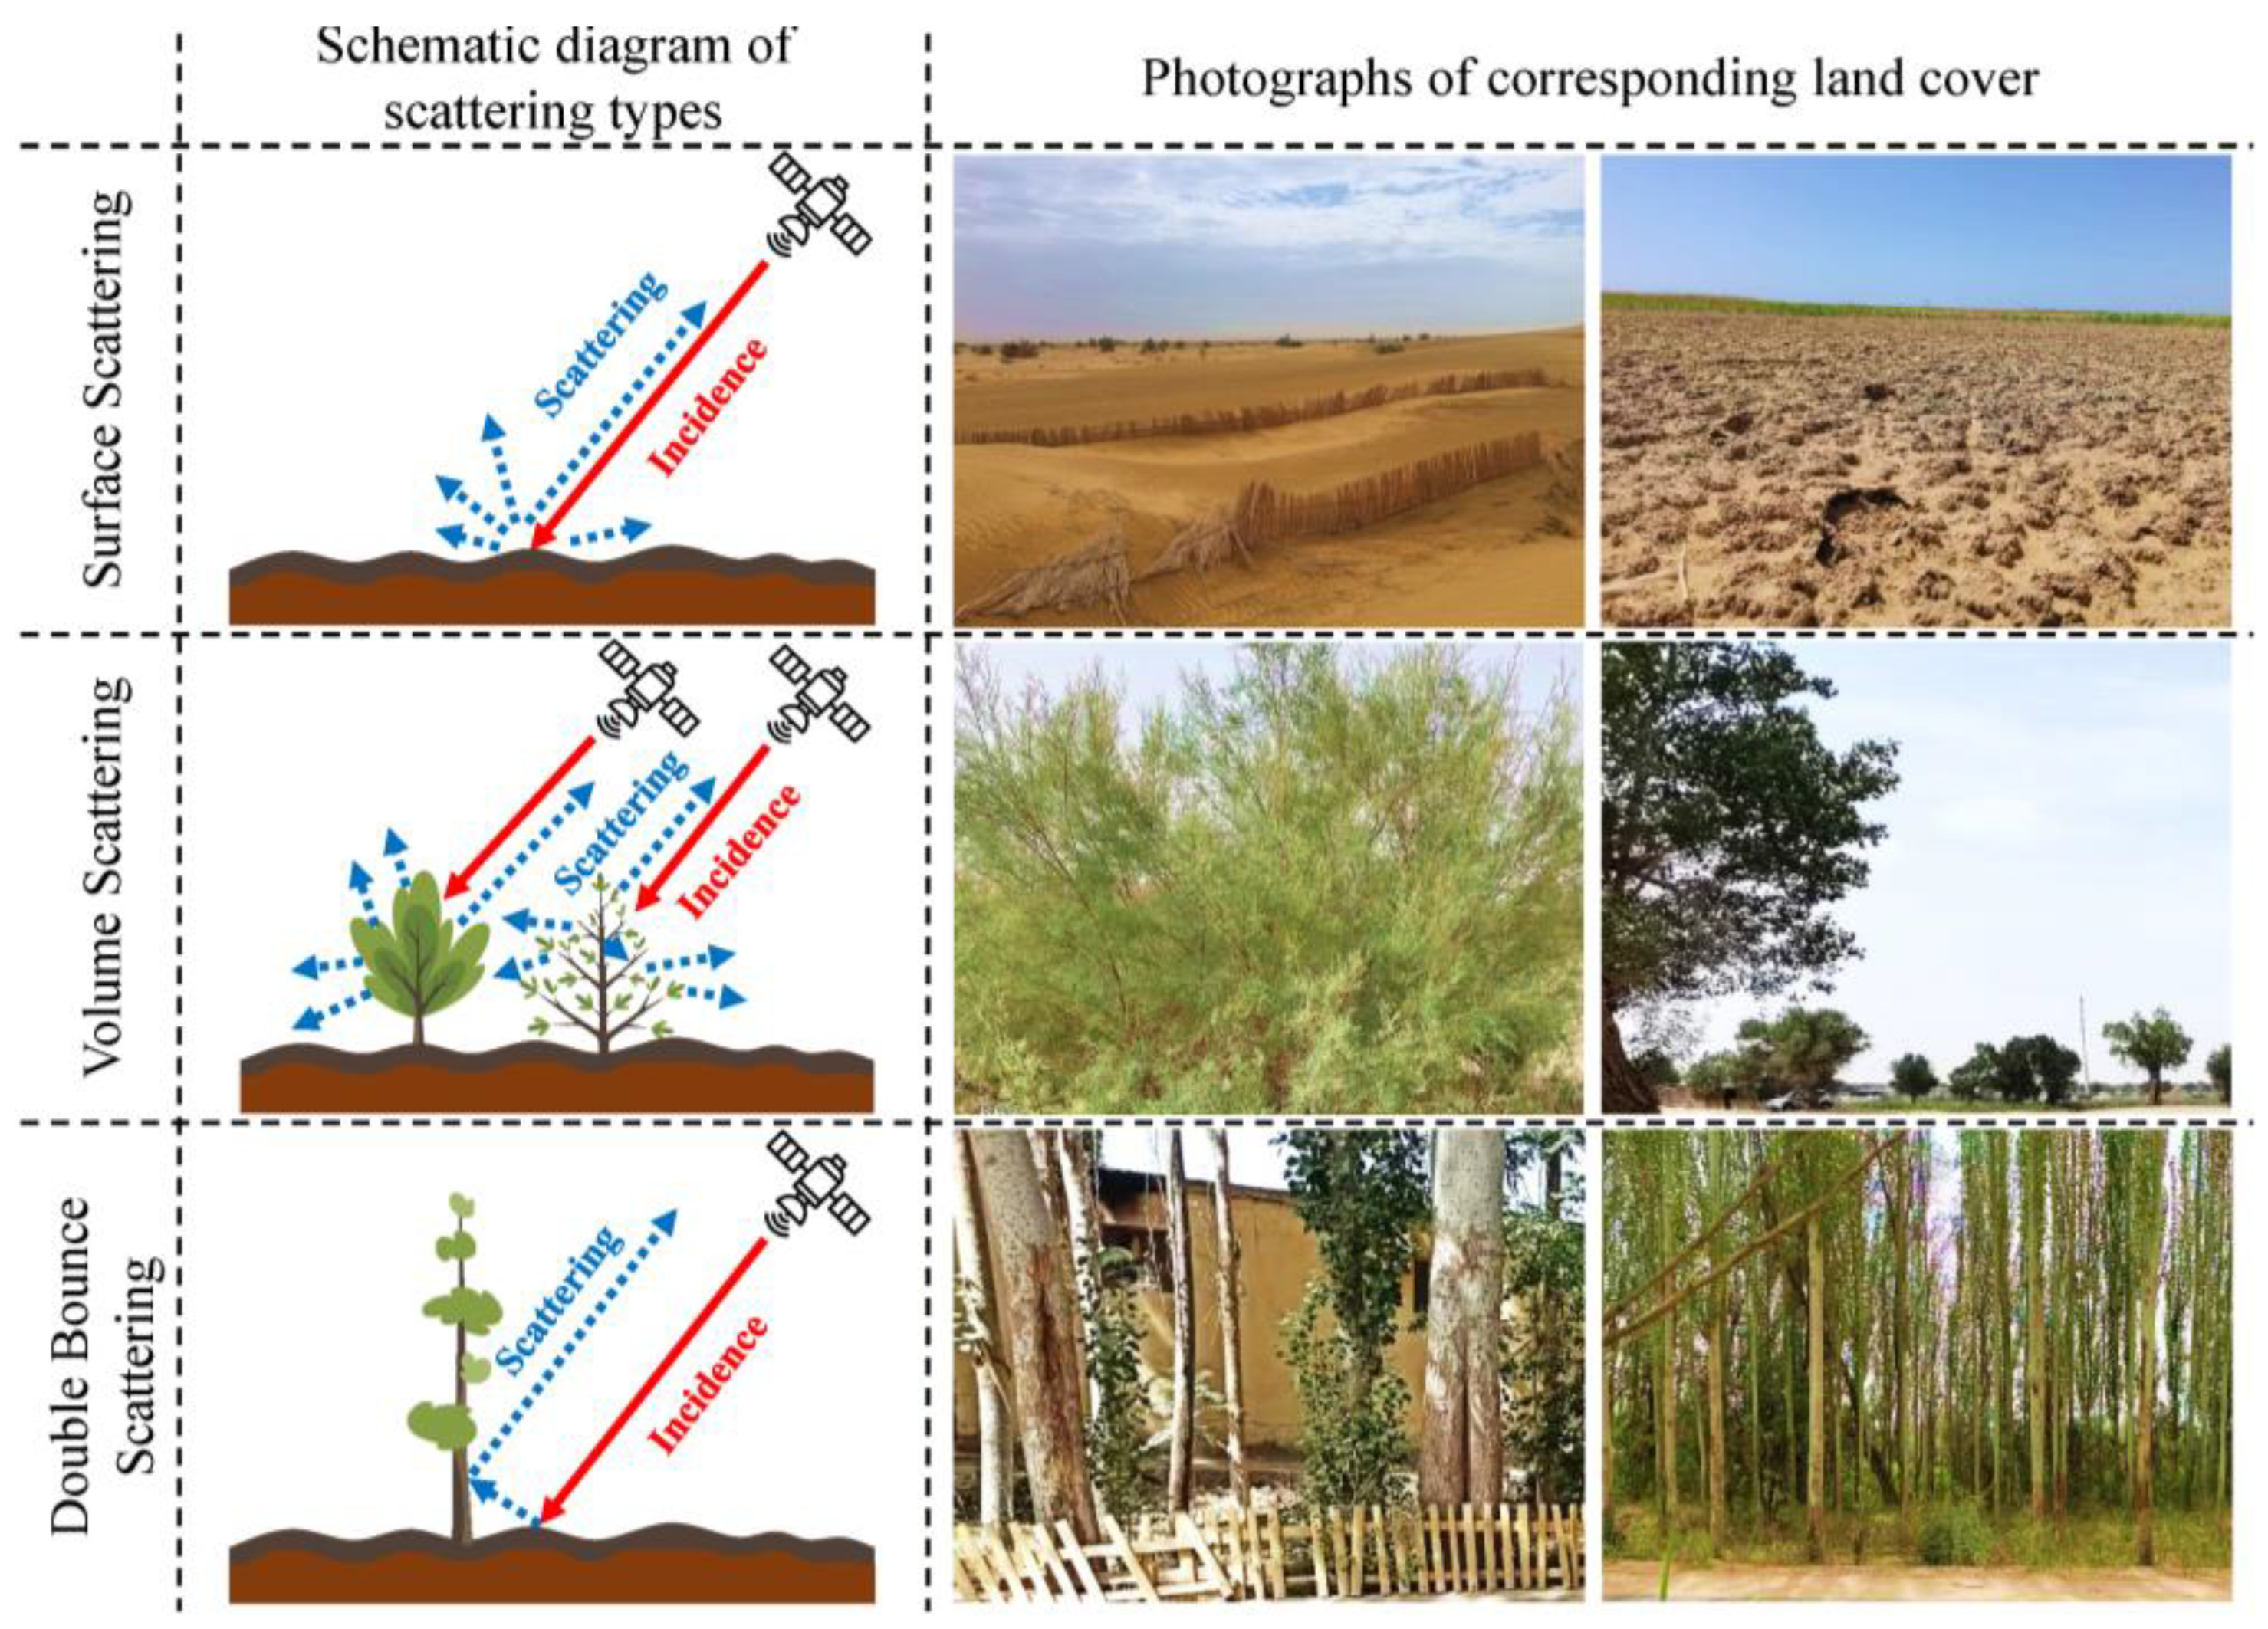
\includegraphics[width=\linewidth,height=0.46\textheight,keepaspectratio]{sensors-25-02512-g003.png}\\[-1pt]
{\tiny Nurmemet et al.\ (2025), \textit{Sensors} 25(8), 2512, doi:10.3390/s25082512}
\scriptsize
\begin{itemize}
\item Bare soil: surface scattering, set by moisture (dielectric) and roughness
\item Canopy: volume and double-bounce scattering mask the soil signal
\end{itemize}
\end{column}
\end{columns}
\end{frame}

\begin{frame}{Motivation\quad Geospatial foundation models (GFMs)}
\centering
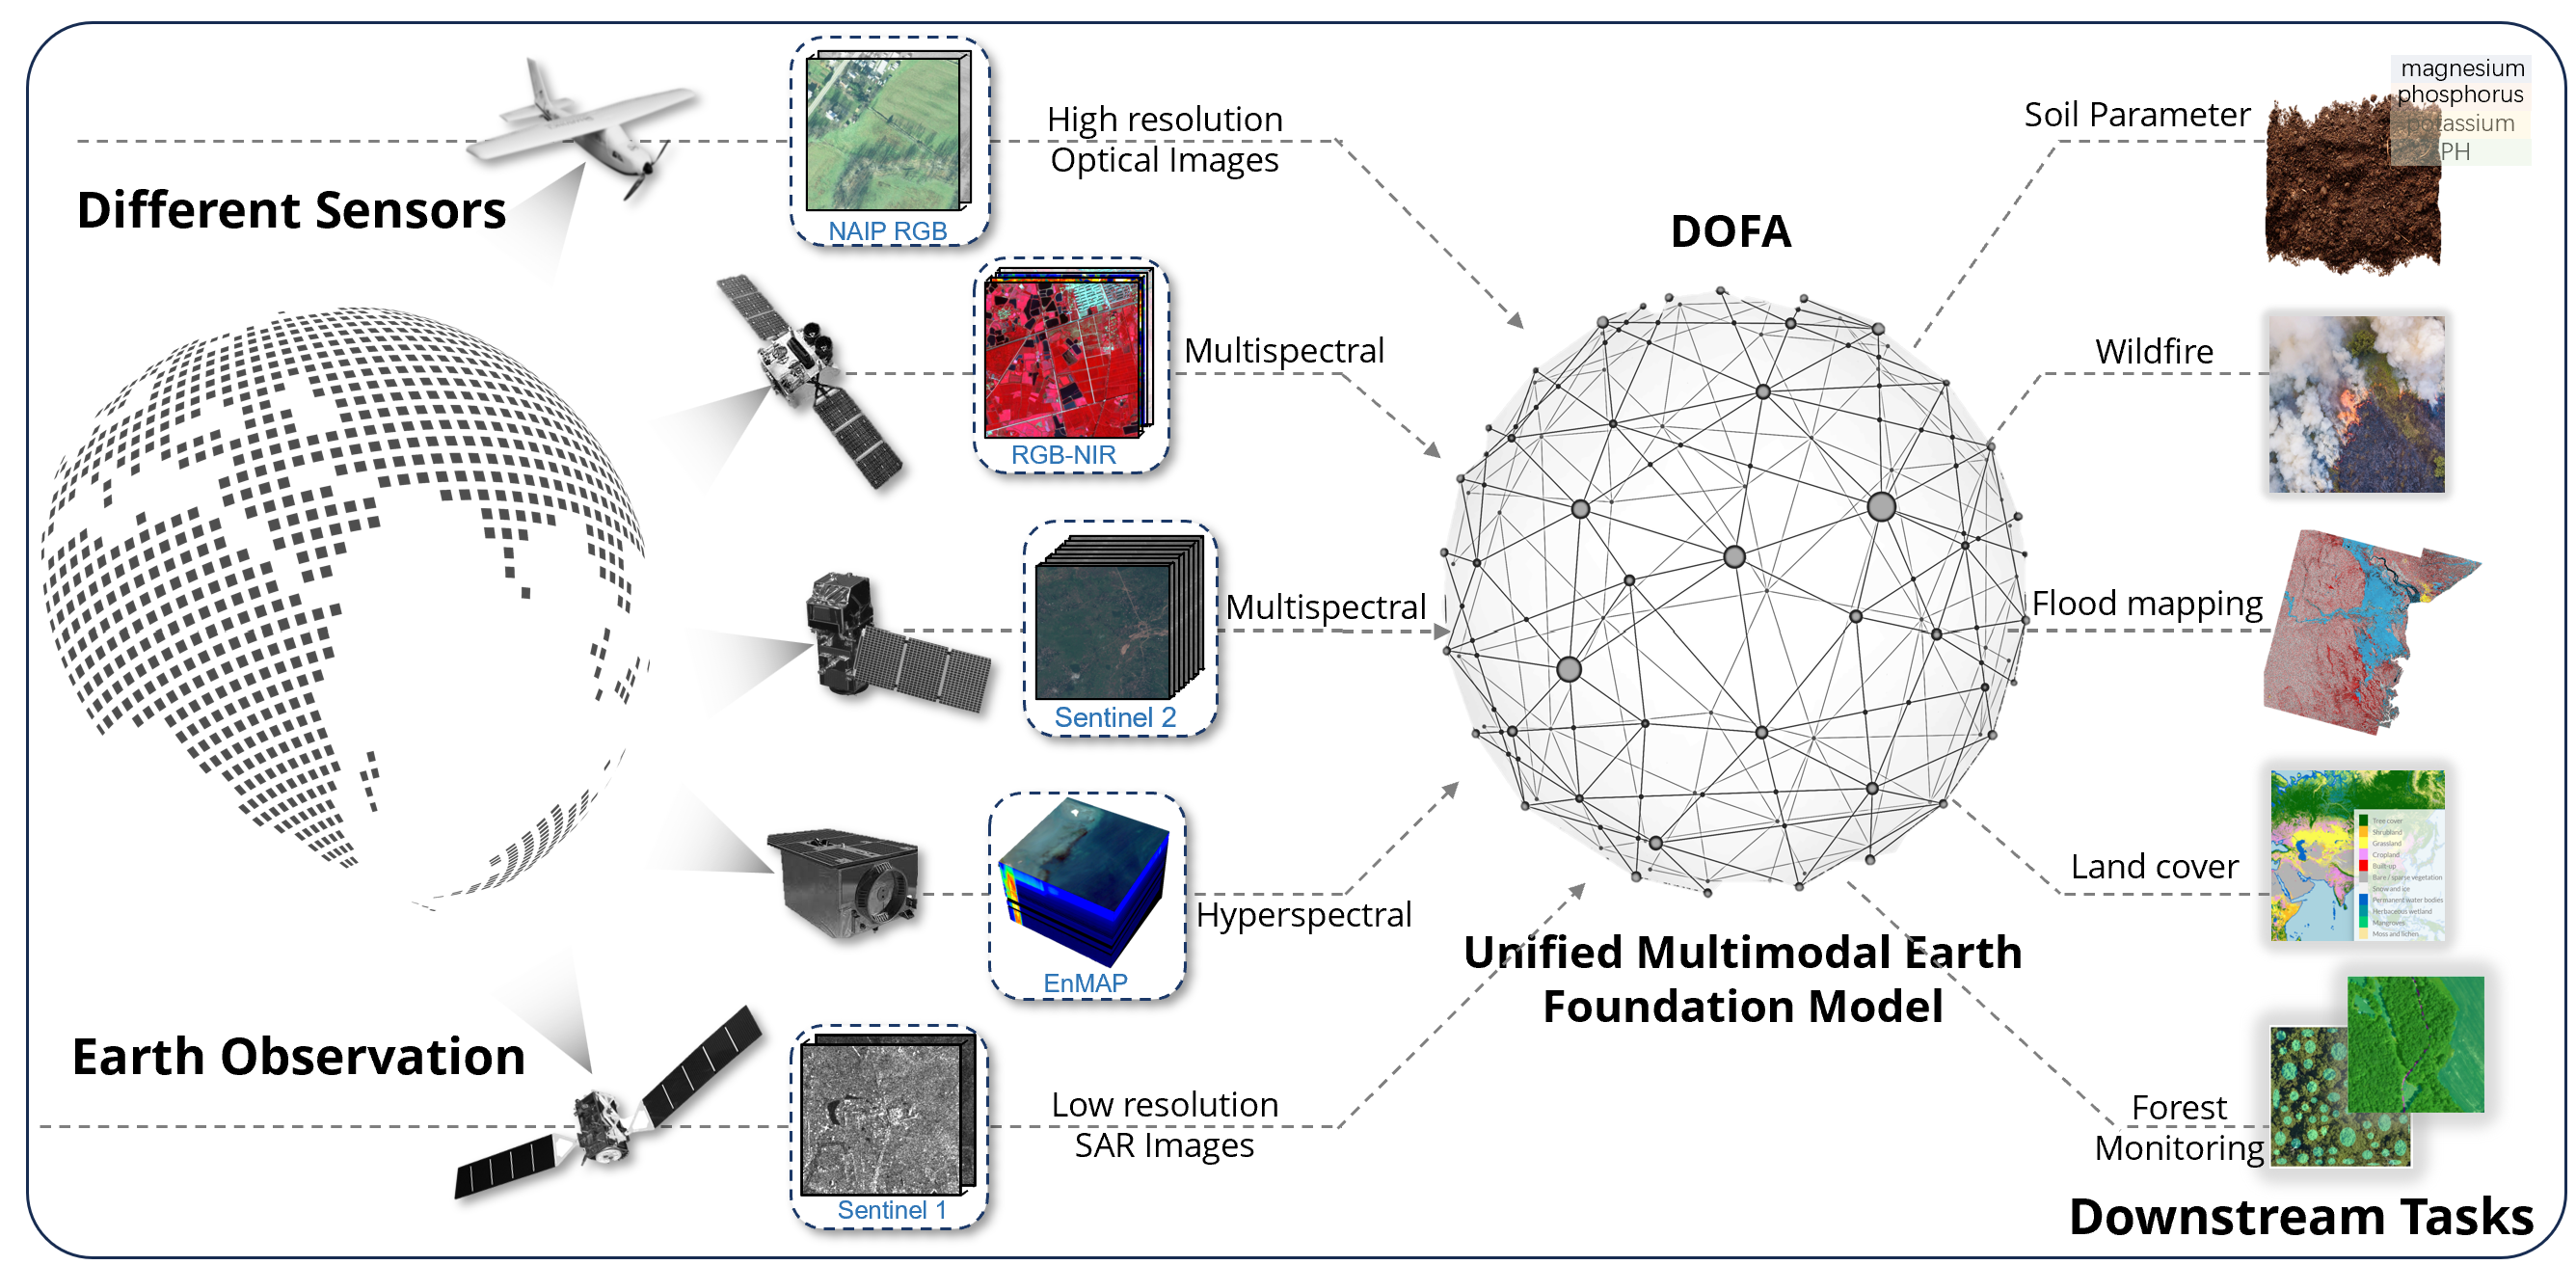
\includegraphics[width=\linewidth,height=0.70\textheight,keepaspectratio]{DOFA1-1.png}\\[-1pt]
{\tiny DOFA: Xiong et al.\ (2024), Neural plasticity-inspired multimodal foundation model for Earth observation, arXiv:2403.15356}\\[6pt]
\begin{beamercolorbox}[wd=0.9\linewidth,center,rounded=true]{block body}
\small\textbf{Once pre-trained on multimodal, unlabelled data, its representation works for many downstream tasks}
\end{beamercolorbox}
\end{frame}

\begin{frame}{Motivation\quad TerraMind embeddings for soil moisture}
\centering
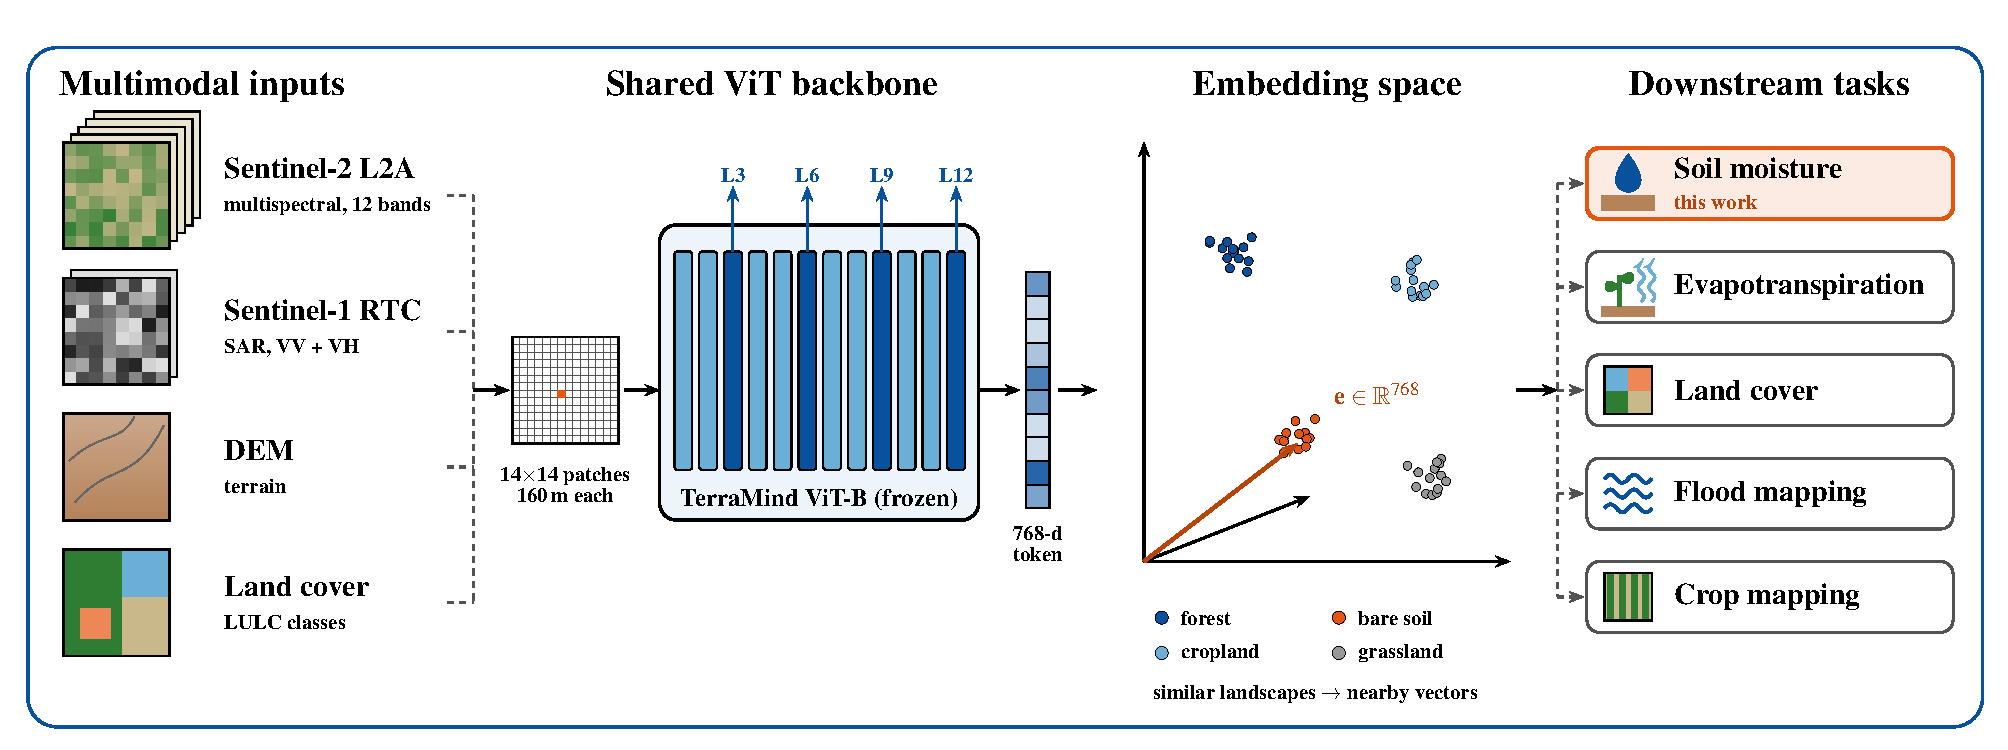
\includegraphics[width=\linewidth,height=0.80\textheight,keepaspectratio]{gfm_embedding_schematic.pdf}\\[4pt]
\footnotesize Frozen TerraMind ViT-B turns each 160\,m patch of S2, S1, DEM and LULC into a 768-d embedding;
the same embedding can serve many tasks; in this case, \textbf{soil moisture}.
\end{frame}



\begin{frame}{Eight research questions}
\footnotesize
\begin{tabular}{@{}l l p{0.62\textwidth}@{}}
\toprule
Block & RQ & Question \\
\midrule
Core      & RQ1 & Do frozen GFM embeddings add skill beyond a multimodal driver baseline? \\
          & RQ2 & What does the model generalise to --- places or processes? \\
          & RQ3 & How does skill vary across the landscape? \\
Mechanism & RQ4 & Which modalities matter, at which depth? \\
          & RQ5 & Does the fine-resolution path carry real sub-km information? \\
Negative  & RQ6 & Is land-surface temperature a useful auxiliary signal for SM? \\
Outlook   & RQ7 & Can the model detect management signals (irrigation)? \\
          & RQ8 & Does the representation transfer to an unseen region? \\
\bottomrule
\end{tabular}
\end{frame}

%---------------- RQ1
\rqslide{RQ1}{Do frozen GFM embeddings add skill beyond a multimodal driver baseline?}
{terramind_value/terramind_value.png}
{TerraMind L12 tokens for S2, S1, DEM and LULC at one tile (TxSON, 2019).}
{\textbf{Have}
\begin{itemize}
\item Modality-shuffle ablation, \S59 model, 221 OOS stations (next slide)
\item Satellite tokens swapped across stations: +37\,\% ubRMSE, $r$ 0.77 $\rightarrow$ 0.52
\end{itemize}
\textbf{Missing}
\begin{itemize}
\item Drivers-only model (10 epochs)
\item Raw-imagery control (GFM vs pixels)
\item Within-station S2 shuffle
\end{itemize}}

\begin{frame}{RQ1\quad What does the model use the GFM embeddings for? (shuffle ablation)}
\scriptsize
\centering
\begin{tabular}{@{}l rr rr rr@{}}
\toprule
 & \multicolumn{2}{c}{0--10 cm} & \multicolumn{2}{c}{10--30 cm} & \multicolumn{2}{c}{30--100 cm} \\
\cmidrule(lr){2-3}\cmidrule(lr){4-5}\cmidrule(l){6-7}
Shuffled input & $\Delta$ubRMSE ($r$) & worse & $\Delta$ubRMSE ($r$) & worse & $\Delta$ubRMSE ($r$) & worse \\
\midrule
All satellite, cross   & +36.8\% (0.52) & 97\% & +37.1\% (0.52) & 96\% & +38.4\% (0.44) & 92\% \\
S2, cross              & +4.9\% (0.74)  & 84\% & +6.8\% (0.72)  & 87\% & +8.7\% (0.63)  & 85\% \\
S1, cross              & +4.8\% (0.73)  & 82\% & +7.7\% (0.70)  & 84\% & +14.4\% (0.58) & 86\% \\
S1, within             & 0.0\% (0.75)   & 49\% & +1.0\% (0.73)  & 59\% & 0.0\% (0.64)   & 49\% \\
DEM, cross             & +12.6\% (0.71) & 90\% & +9.7\% (0.68)  & 86\% & +18.4\% (0.59) & 96\% \\
LULC, cross            & +6.1\% (0.73)  & 82\% & +6.6\% (0.70)  & 82\% & +12.7\% (0.62) & 87\% \\
Fine 20 m path, cross  & +0.5\% (0.75)  & 56\% & +1.3\% (0.74)  & 65\% & +0.1\% (0.68)  & 52\% \\
\midrule
ERA5, cross            & +30.3\% (0.50) & 95\% & +24.6\% (0.54) & 91\% & +15.1\% (0.50) & 86\% \\
ERA5, within           & +39.0\% (0.35) & 88\% & +30.4\% (0.37) & 81\% & +13.5\% (0.34) & 73\% \\
Soil, cross            & +7.6\% (0.72)  & 87\% & +17.6\% (0.63) & 92\% & +25.7\% (0.55) & 94\% \\
SIF, cross             & +1.3\% (0.75)  & 63\% & +1.6\% (0.73)  & 62\% & +1.8\% (0.67)  & 71\% \\
TWSA, cross            & 0.0\% (0.77)   & 50\% & 0.0\% (0.76)   & 53\% & +0.1\% (0.71)  & 58\% \\
\bottomrule
\end{tabular}

\vspace{4pt}
\raggedright
Baseline: ubRMSE 0.050 / 0.048 / 0.048, $r$ 0.766 / 0.761 / 0.702 ($n$ = 221 / 144 / 119).
\emph{Cross} = another station's input (kills site identity); \emph{within} = same station, shuffled dates (kills timing).
\end{frame}

\begin{frame}{RQ1\quad What we can and cannot claim today}
\footnotesize
\begin{columns}[T,onlytextwidth]
\begin{column}{0.55\textwidth}
\textbf{Can claim}
\begin{enumerate}
\item Reliance on GFM tokens $\approx$ reliance on weather (+37\,\% vs +30\,\%).
\item Tokens are a \emph{static landscape descriptor}: S1 within-station shuffle = 0\,\%.
\item They shape the response, not just the mean (ubRMSE is bias-free): \emph{GFM embeddings condition the weather$\rightarrow$SM transfer on the landscape.}
\item Depth pattern inverted vs a moisture signal: S1 +4.8\,\% $\rightarrow$ +14.4\,\% with depth.
\item Modalities redundant: S2+S1+DEM+LULC $\approx$ 28\,\% $<$ 37\,\% joint.
\item Fine 20\,m path and TWSA unused.
\end{enumerate}
\end{column}
\begin{column}{0.42\textwidth}
\textbf{Cannot claim yet}
\begin{itemize}
\item \emph{Added} skill --- a shuffle measures reliance
\item GFM better than raw imagery
\item Anything about S2 dynamics
\end{itemize}
\textbf{To answer fully}
\begin{itemize}
\item Within-station S2 shuffle (eval only)
\item Run A: drivers + soil, no tokens
\item Run B: A + static site descriptors
\item Full $>$ B $>$ A $\Rightarrow$ dynamic skill;\\ Full $\approx$ B $>$ A $\Rightarrow$ site info only
\end{itemize}
\end{column}
\end{columns}
\end{frame}

%---------------- RQ2
\rqslide{RQ2}{What does the model generalise to --- places or processes?}
{eval/box_ubrmse_by_kg_macro.png}
{Per-station ubRMSE by climate zone and split (OOS / OOT / OOST).}
{\textbf{Have}
\begin{itemize}
\item Splits \S47: train 573 / val 89 / OOS 224; OOT 2023--2025
\item OOT error is \emph{lower} than OOS in every climate zone: new years at known sites are easy, new sites are hard
\item \texttt{pw\_stage2a\_L3}: OOT 0.0434 beat val 0.0507
\item Step-0 offsets probe: pair sign 0.50; site-fingerprint verdict confirmed (27572594)
\end{itemize}
\textbf{Missing}
\begin{itemize}
\item One val / OOT / OOS table for the selected model
\end{itemize}}

%---------------- RQ3
\rqslide{RQ3}{How does skill vary across the landscape?}
{eval/box_ubrmse_by_igbp_macro.png}
{Per-station ubRMSE by land-cover class and split.}
{\textbf{Have}
\begin{itemize}
\item Per-station metrics by climate zone and land cover
\item LULC, elevation band, soil, HAND for every station
\item HAND stable under DEM noise; TWI is not --- use HAND
\end{itemize}
\textbf{Missing}
\begin{itemize}
\item Error vs aridity, HAND, soil texture, per depth
\item Flag elevation sentinels first (18 REMEDHUS = $-$99.9, Baytik = 0)
\end{itemize}}

%---------------- RQ4
\rqslide{RQ4}{Which modalities matter, at which depth?}
{eval/box_ubrmse_by_depth.png}
{Per-station ubRMSE by depth.}
{\textbf{Have} (shuffle ablation, RQ1 table)
\begin{itemize}
\item ERA5 dynamics dominate the surface (+39\,\%) and fade with depth (+14\,\%)
\item Soil properties grow with depth (+7.6\,\% $\rightarrow$ +25.7\,\%)
\item SIF $\approx$ 1.5\,\%; TWSA $\approx$ 0
\item \S58: 180-day ERA5 window
\end{itemize}
\textbf{Hypothesis status}
\begin{itemize}
\item ``TWSA drives the root zone'' --- not supported so far
\end{itemize}}

%---------------- RQ5
\rqslide{RQ5}{Does the fine-resolution path carry real sub-kilometre information?}
{effres/effres_txson.png}
{Effective-resolution test at TxSON (\S70).}
{\textbf{Have}
\begin{itemize}
\item \S53 fine ablation: SM ignores the 20\,m path (LST reads it)
\item Fine-path shuffle: +0.1 to +1.3\,\% ubRMSE
\item \S48 map flattens after epoch 8
\item Overijssel grid run (\S68, paused)
\end{itemize}
\textbf{Framing}
\begin{itemize}
\item A publishable negative result if framed well
\end{itemize}}

%---------------- RQ6
\rqslide{RQ6}{Is land-surface temperature a useful auxiliary signal for soil moisture?}
{tile_lst_seasonal/ISMN_TxSON_CR200-18.png}
{Within-tile Landsat LST anomaly by month, TxSON CR200-18 (\S29).}
{\textbf{Have (all negative)}
\begin{itemize}
\item Within-tile LST pattern is static: $r$ = +0.967 across months
\item Simpson's paradox: +0.167 pooled, $-$0.077 within station
\item ECOSTRESS DTR = day pattern ($r$ = +0.816); G0 fails
\item In training LST hurts SM: val 0.0537 with vs 0.0487 without
\end{itemize}
\textbf{Status}
\begin{itemize}
\item Ready to write as a short paper / section
\end{itemize}}

%---------------- RQ7
\rqslide{RQ7}{Can the model detect management signals such as irrigation?}
{mead/mead_pw_sm_2017-2024.png}
{Mead Ne1/Ne2/Ne3: model vs observed SM, 2017--2024 (\S69).}
{\textbf{Have}
\begin{itemize}
\item Mead daily SM built for Ne1/Ne2/Ne3
\item Irrigation visible only in the dry year (2022)
\end{itemize}
\textbf{Missing}
\begin{itemize}
\item Irrigation log covers 2014--2021 only
\item Prediction-minus-observation analysis vs irrigation dates
\end{itemize}}

%---------------- RQ8
\rqslide{RQ8}{Does the representation transfer to an unseen region?}
{nl_grid/nl_tiles.png}
{Overijssel grid tiles (\S68).}
{\textbf{Have}
\begin{itemize}
\item Overijssel: cloud mask done 688/688
\item TWENTE: 8 stations, all OOS (end 2020, no OOT)
\end{itemize}
\textbf{Missing}
\begin{itemize}
\item Prep $\rightarrow$ tokenise $\rightarrow$ post $\rightarrow$ predict
\item Map + TWENTE station comparison
\end{itemize}}

\end{document}
